\subsubsection{Filtrage simple}

\begin{figure}[H]
    \begin{center}
    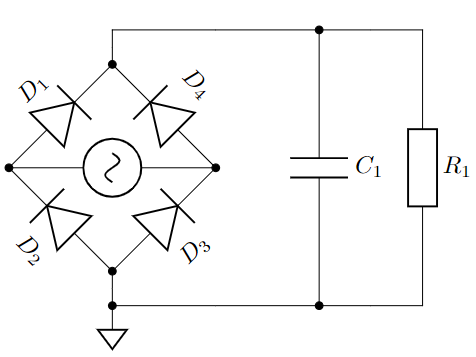
\includegraphics[scale=0.5]{images/5.png}
    \caption{Filtrage simple}
    \end{center}
\end{figure}

Nous avons reproduis le circuit précédent sur LTSPICE, voici son rendu : 

\begin{figure}[H]
    \begin{center}
    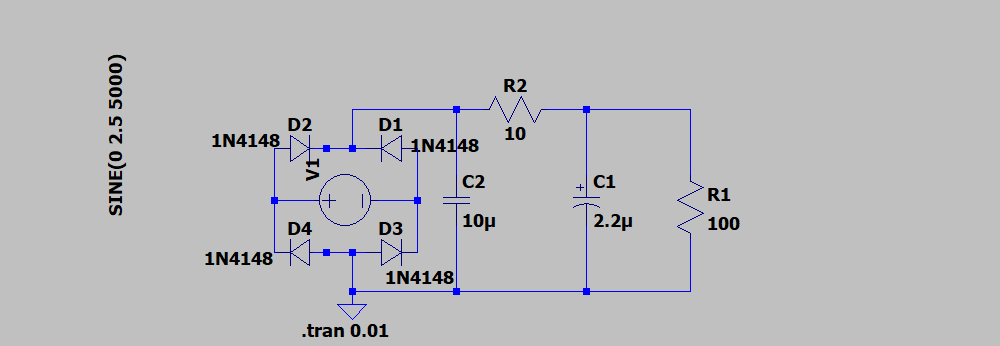
\includegraphics[scale=0.4]{images/LTSPICE/1.png}
    \caption{Filtrage simple sur LTSPICE}
    \end{center}
\end{figure}

Ensuite, nous représenté l’allure de la tension aux bornes de $R_1$ sur $10 ms$ avec différentes valeurs de $R_1$ : $10k\Omega$ ; $5.6k\Omega$ ;
$2.2k\Omega$ ; $1k\Omega$ ; $560\Omega$ ; $220\Omega$ ; $100\Omega$, que voici : 

\begin{figure}[H]
    \begin{center}
    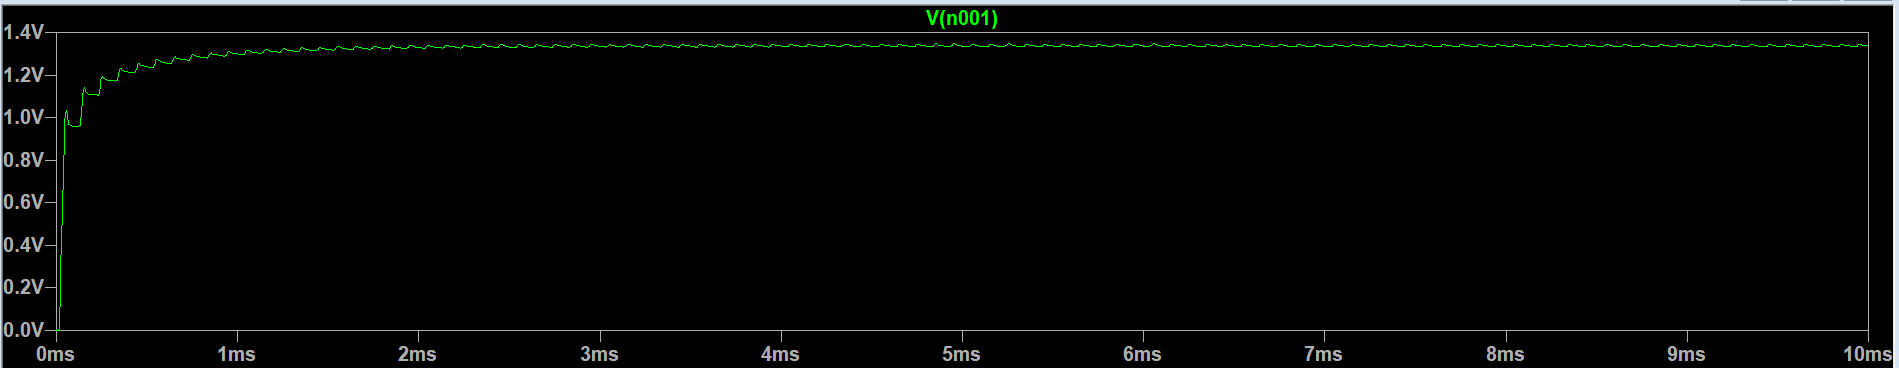
\includegraphics[scale=0.25]{images/LTSPICE/2.png}
    \caption{$R=10k\Omega$}
    \end{center}
\end{figure}

\begin{figure}[H]
    \begin{center}
    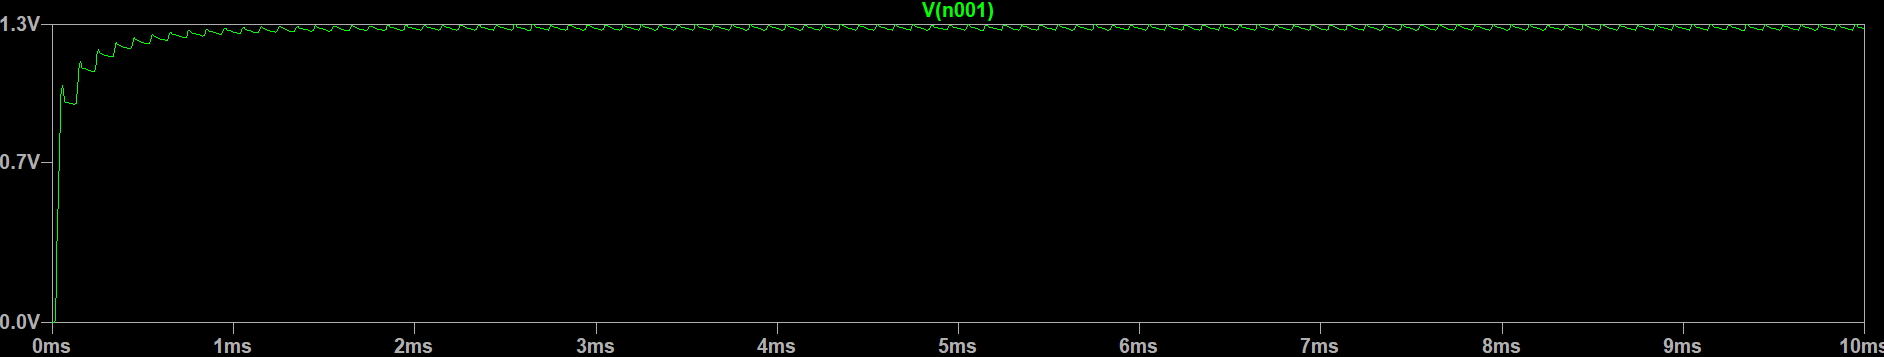
\includegraphics[scale=0.25]{images/LTSPICE/3.png}
    \caption{$R=5.6k\Omega$}
    \end{center}
\end{figure}

\begin{figure}[H]
    \begin{center}
    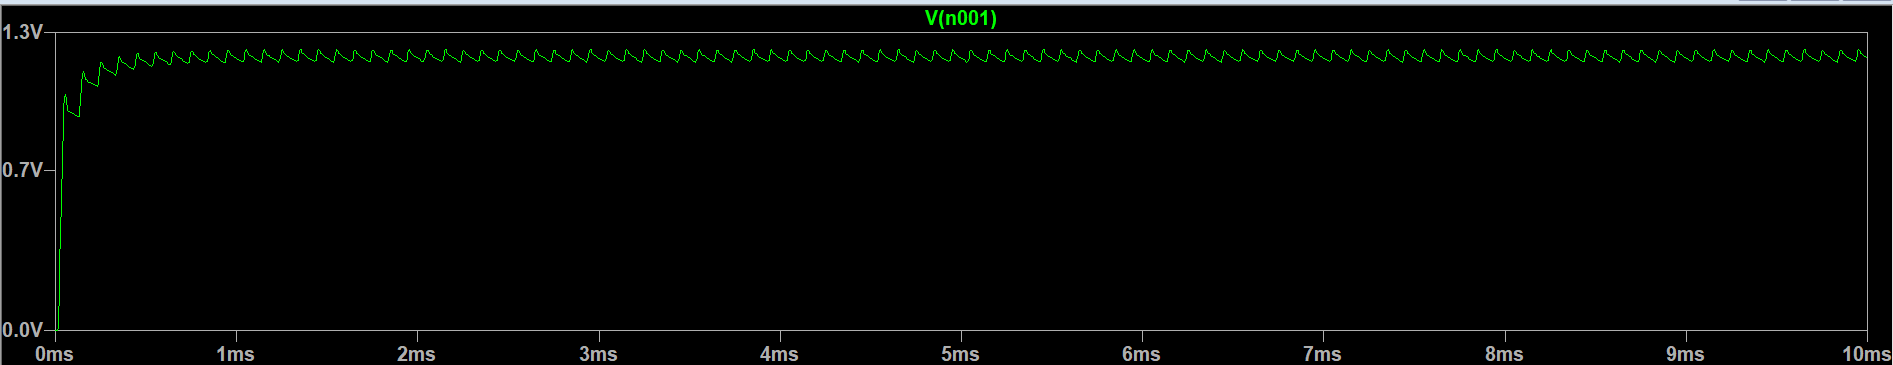
\includegraphics[scale=0.25]{images/LTSPICE/4.png}
    \caption{$R=2.2k\Omega$}
    \end{center}
\end{figure}

\begin{figure}[H]
    \begin{center}
    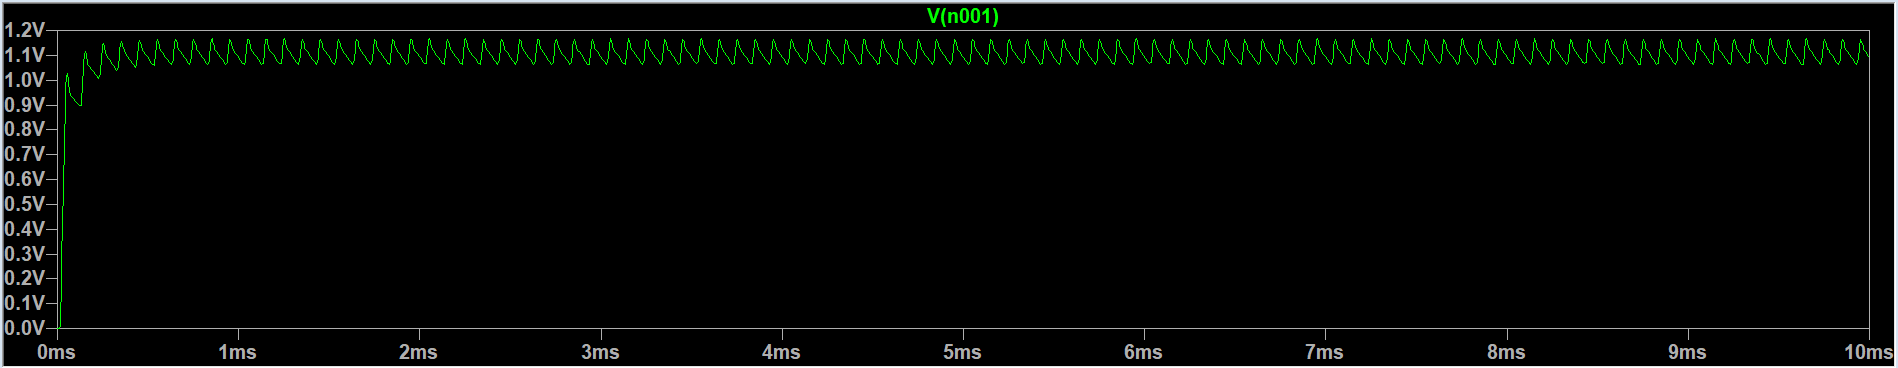
\includegraphics[scale=0.25]{images/LTSPICE/5.png}
    \caption{$R=1k\Omega$}
    \end{center}
\end{figure}

\begin{figure}[H]
    \begin{center}
    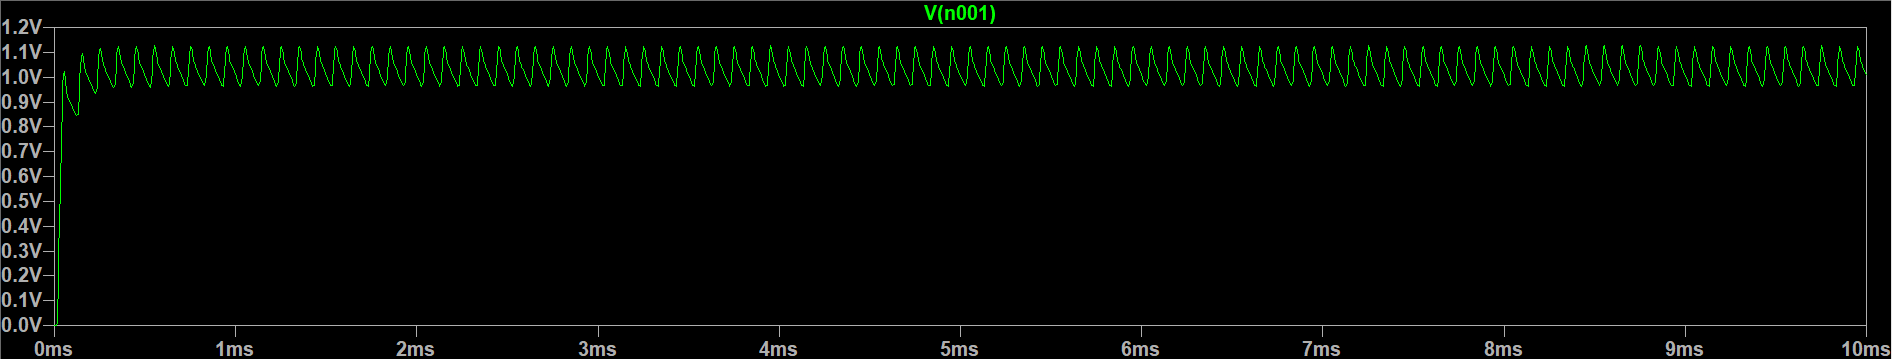
\includegraphics[scale=0.25]{images/LTSPICE/6.png}
    \caption{$R=560\Omega$}
    \end{center}
\end{figure}

\begin{figure}[H]
    \begin{center}
    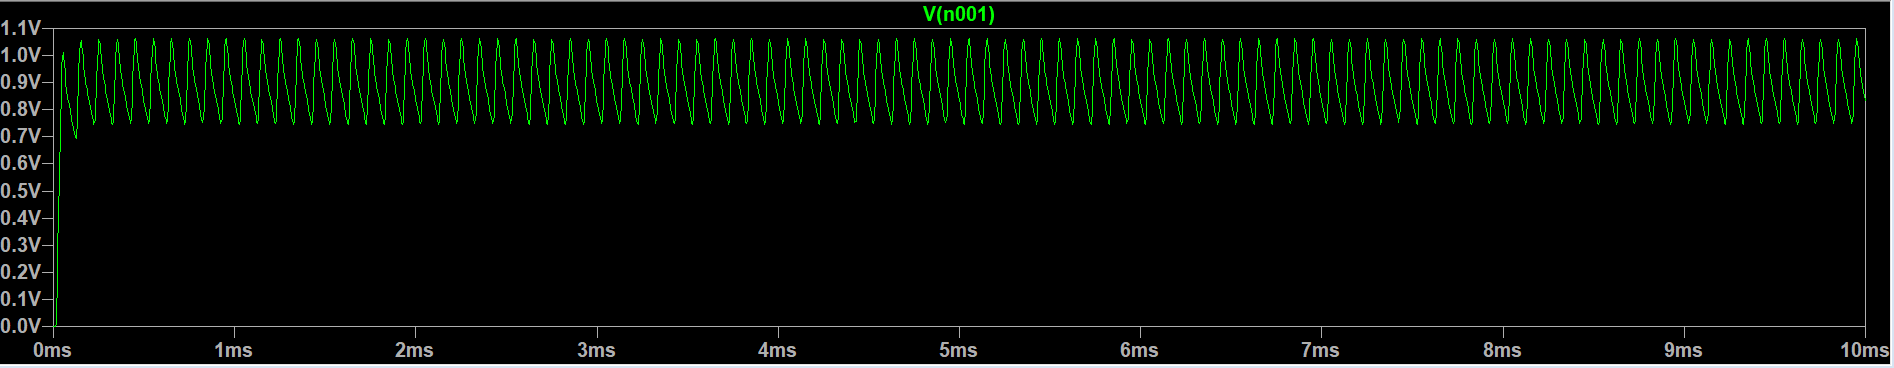
\includegraphics[scale=0.25]{images/LTSPICE/7.png}
    \caption{$R=220\Omega$}
    \end{center}
\end{figure}

\begin{figure}[H]
    \begin{center}
    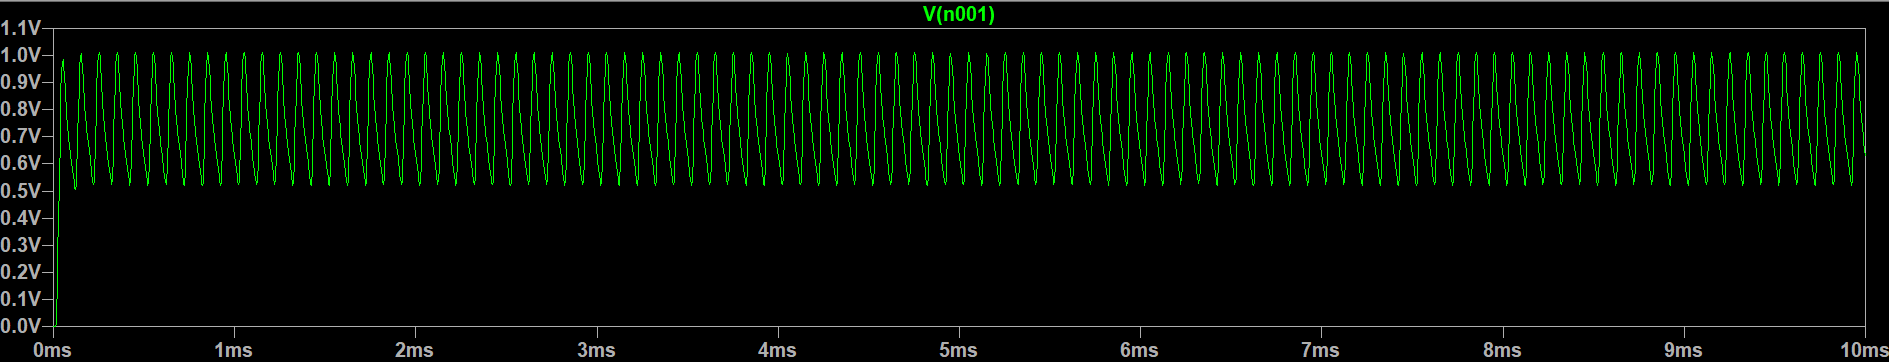
\includegraphics[scale=0.25]{images/LTSPICE/8.png}
    \caption{$R=100\Omega$}
    \end{center}
\end{figure}

Nous pouvons en conclure que lorsque $R_1$ diminue, le signal oscille de plus en plus et la tension maximale diminue.


\subsubsection{Filtrage double}

\begin{figure}[H]
    \begin{center}
    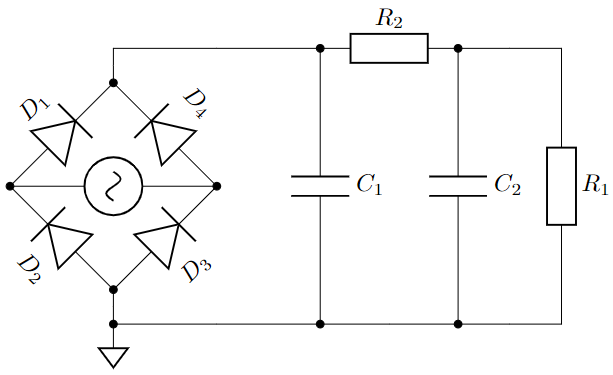
\includegraphics[scale=0.5]{images/6.png}
    \caption{Filtrage double}
    \end{center}
\end{figure}

Nous avons reproduis le circuit précédent sur LTSPICE, voici son rendu :

\begin{figure}[H]
    \begin{center}
    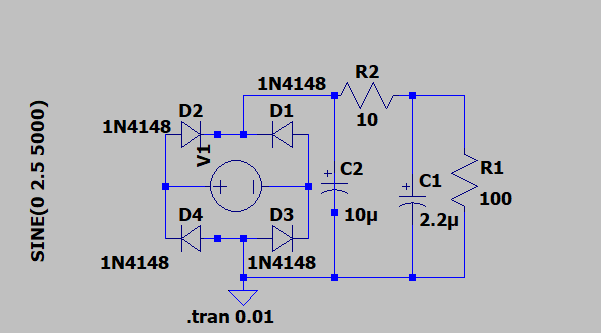
\includegraphics[scale=0.4]{images/LTSPICE/a.png}
    \caption{Filtrage double sur LTSPICE}
    \end{center}
\end{figure}

Ensuite, nous représenté l’allure de la tension aux bornes de $R_1$ sur $10 ms$ avec différentes valeurs de $R_1$ : $10k\Omega$ ; $5.6k\Omega$ ; $2.2k\Omega$ ; $1k\Omega$ ; $560\Omega$ ; $220\Omega$ ; $100\Omega$, que voici : 

\begin{figure}[H]
    \begin{center}
    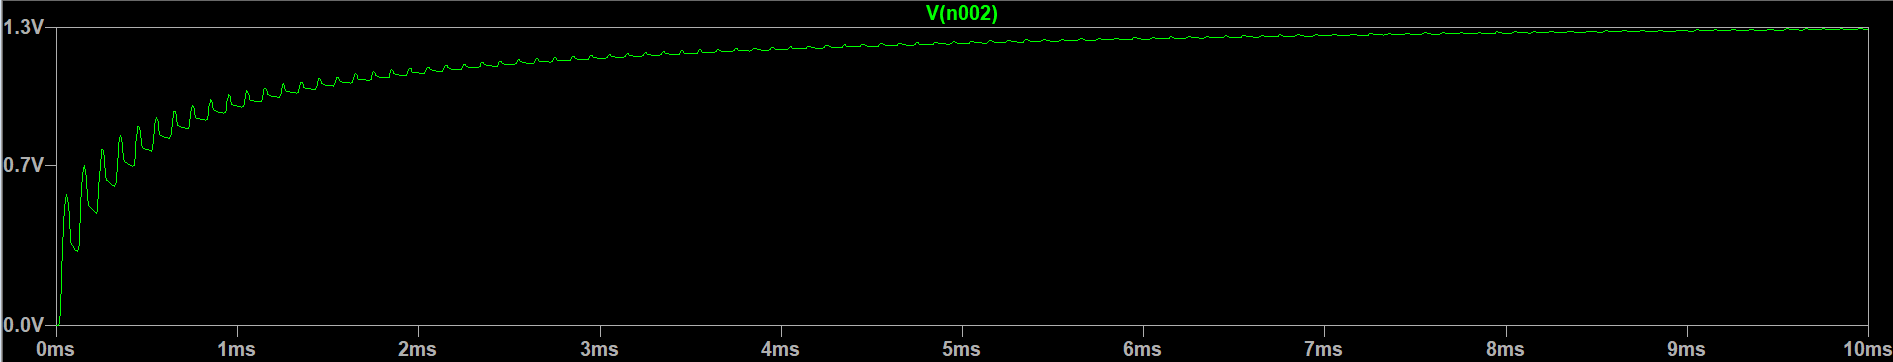
\includegraphics[scale=0.25]{images/LTSPICE/b.png}
    \caption{$R=10k\Omega$}
    \end{center}
\end{figure}

\begin{figure}[H]
    \begin{center}
    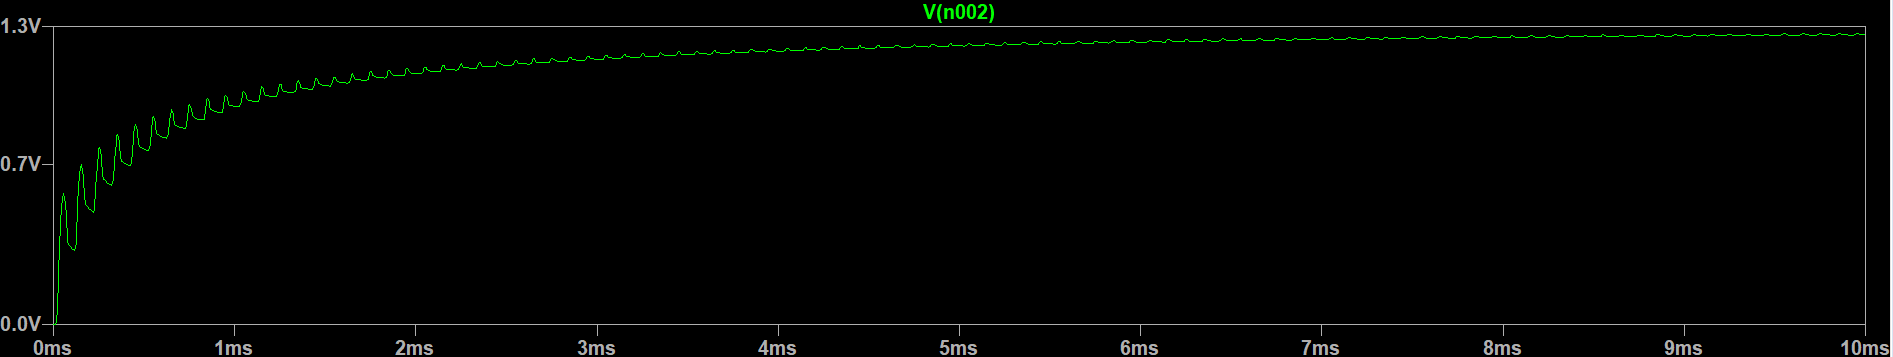
\includegraphics[scale=0.25]{images/LTSPICE/c.png}
    \caption{$R=5.6k\Omega$}
    \end{center}
\end{figure}

\begin{figure}[H]
    \begin{center}
    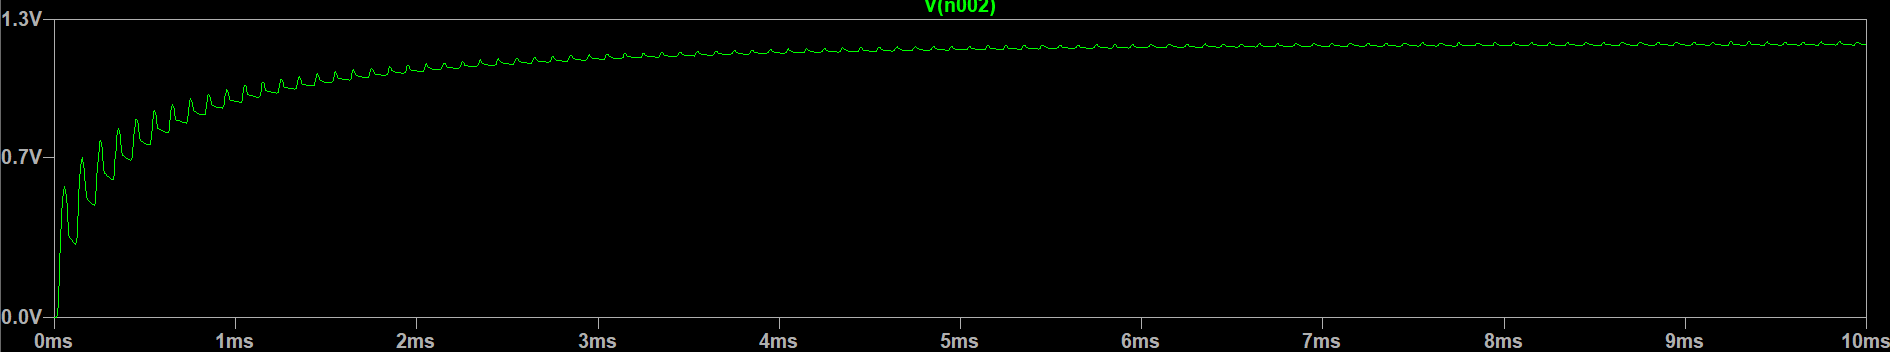
\includegraphics[scale=0.25]{images/LTSPICE/d.png}
    \caption{$R=2.2k\Omega$}
    \end{center}
\end{figure}

\begin{figure}[H]
    \begin{center}
    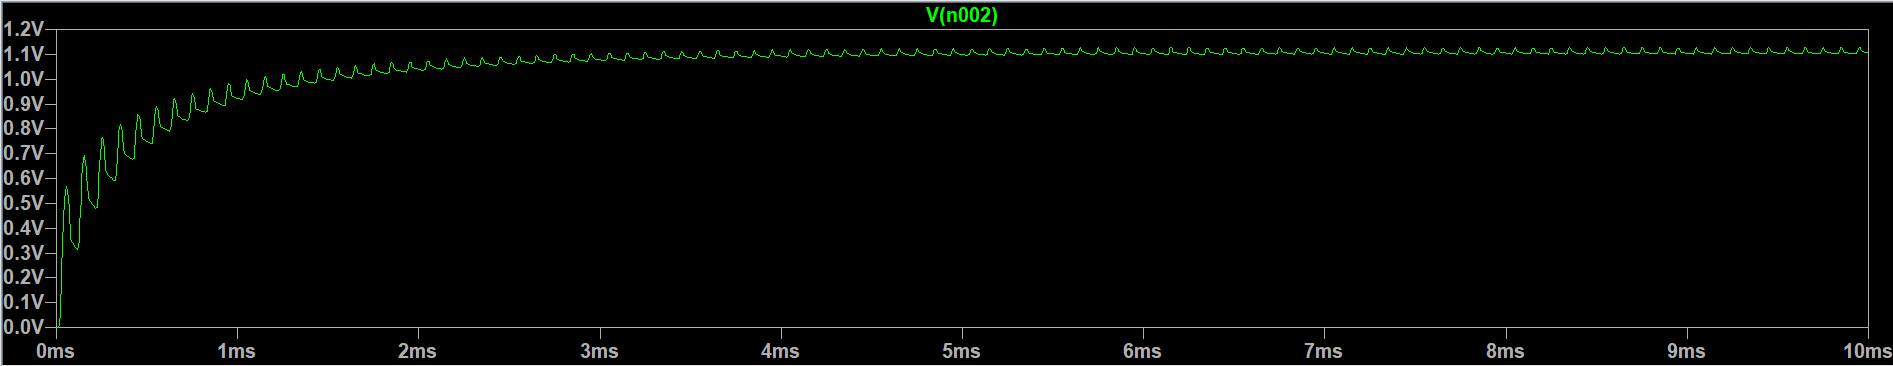
\includegraphics[scale=0.25]{images/LTSPICE/e.png}
    \caption{$R=1k\Omega$}
    \end{center}
\end{figure}

\begin{figure}[H]
    \begin{center}
    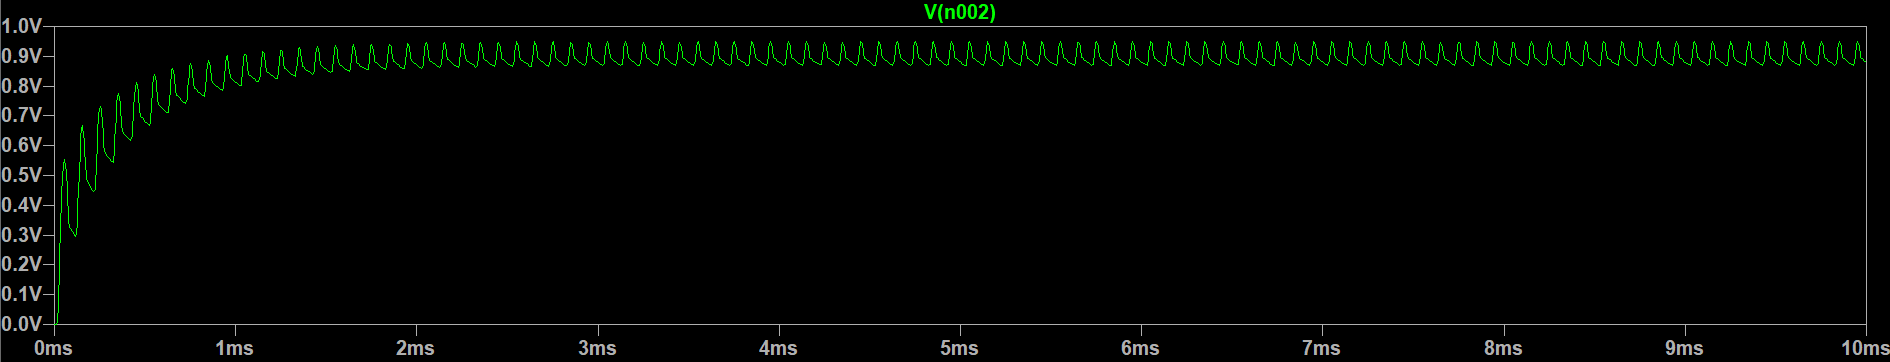
\includegraphics[scale=0.25]{images/LTSPICE/f.png}
    \caption{$R=560\Omega$}
    \end{center}
\end{figure}

\begin{figure}[H]
    \begin{center}
    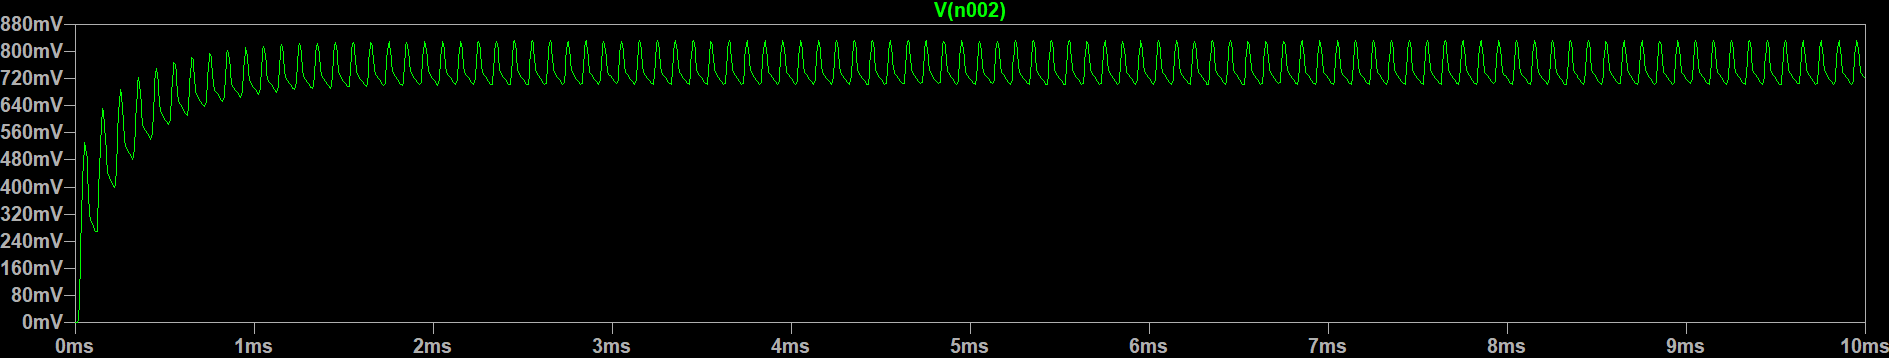
\includegraphics[scale=0.25]{images/LTSPICE/g.png}
    \caption{$R=220\Omega$}
    \end{center}
\end{figure}

Nous pouvons voir que le signal est meilleur qu'avant : cela est dû au fait que le filtrage double est plus efficace que le filtrage simple, avec les deux condensateurs en parallèle.
\\
Cependant, le principal inconveniant de ce montage est que le signal est déphasé de $\frac{\pi}{2}$, ce qui peut poser problème dans certaines applications. De plus, il est nécessaire d'avoir un composants suplémentaire.